\documentclass{acm_proc_article-sp}

\usepackage[utf8]{inputenc}
\usepackage[T1]{fontenc}

\usepackage[activate=compatibility]{microtype}

% autoref command
\usepackage[pdftex,urlcolor=black,colorlinks=true,linkcolor=black,citecolor=black]{hyperref}
\def\sectionautorefname{Section}
\def\subsectionautorefname{Subsection}
\def\subfloatautorefname{Subfigure}

\usepackage[lofdepth,lotdepth]{subfig}

\usepackage{enumitem}

\usepackage{mathtools}

% give emph a normal fontsize
\let\oldemph\emph
\renewcommand{\emph}[1]{\oldemph{\fontsize{9}{9}\selectfont #1}}

% more readable footnote layout
\renewcommand{\footnotesize}{\fontsize{8pt}{10pt}}
\setlength{\footnotesep}{.5cm}

% todo macro
\usepackage{color}
\newcommand{\todo}[1]{\noindent\textcolor{red}{{\bf \{TODO}: #1{\bf \}}}}

% listings and Verbatim environment
\usepackage{fancyvrb}
\usepackage{relsize}
\usepackage{listings}
\usepackage{verbatim}
\newcommand{\defaultlistingsize}{\fontsize{8pt}{9.5pt}}
\newcommand{\inlinelistingsize}{\fontsize{8pt}{11pt}}
\newcommand{\smalllistingsize}{\fontsize{7.5pt}{9.5pt}}
\newcommand{\listingsize}{\defaultlistingsize}
\RecustomVerbatimCommand{\Verb}{Verb}{fontsize=\inlinelistingsize}
\RecustomVerbatimEnvironment{Verbatim}{Verbatim}{fontsize=\defaultlistingsize}
\lstset{frame=lines,captionpos=b,numberbychapter=false,escapechar=§,
        aboveskip=0.5em,belowskip=0em,abovecaptionskip=0em,belowcaptionskip=0em,
framexbottommargin=-1em,
        basicstyle=\ttfamily\listingsize\selectfont}

% use Courier from this point onward
\let\oldttdefault\ttdefault
\renewcommand{\ttdefault}{pcr}
\let\oldurl\url
\renewcommand{\url}[1]{\inlinelistingsize\oldurl{#1}}

% superscript for 1st, 2nd, etc.
%\newcommand{\superscript}[1]{\ensuremath{^{\textrm{#1}}}}
%\newcommand{\subscript}[1]{\ensuremath{_{\textrm{#1}}}}
%\newcommand{\th}[0]{\superscript{th}}
%\newcommand{\st}[0]{\superscript{st}}
%\newcommand{\nd}[0]{\superscript{nd}}
%\newcommand{\rd}[0]{\superscript{rd}}

% linewrap symbol
\definecolor{grey}{RGB}{130,130,130}
\newcommand{\linewrap}{\raisebox{-.6ex}{\textcolor{grey}{$\hookleftarrow$}}}

% more pleasing quote environment
\usepackage{tikz}
\newcommand*{\openquote}{\tikz[remember picture,overlay,xshift=-7pt,yshift=1pt]
     \node (OQ) {\fontfamily{fxl}\fontsize{16}{16}\selectfont``};\kern0pt}
\newcommand*{\closequote}{\tikz[remember picture,overlay,xshift=2pt,yshift=-4.5pt]
     \node (CQ) {\fontfamily{fxl}\fontsize{16}{16}\selectfont''};}
\renewenvironment{quote}%
{\setlength{\parindent}{1cm}\par\openquote}
{\closequote\vspace{-4.5pt}
}

\makeatletter
\let\@copyrightspace\relax
\makeatother

\begin{document}

\title{Getting the Bigger Picture -- Extracting Media Items Covering Events from Multiple Social Networks}

\numberofauthors{3}
\author{
\alignauthor
\textbf{Thomas Steiner}\\
	\affaddr{Google Germany GmbH}\\
	\affaddr{tomac@google.com}
\alignauthor
\textbf{Raphaël Troncy}\\
	\affaddr{EURECOM}\\
	\affaddr{rtroncy@eurecom.fr}
\alignauthor
\textbf{Ruben Verborgh}\\ 	
	\affaddr{UGhent}\\
	\affaddr{ruben.verborgh@ughent.be}
}

\maketitle

\begin{abstract}

\end{abstract}

\category{H.3.4}{Information Systems}{Information Storage and Retrieval}[World Wide Web]
\category{H.3.5}{Online Information Services}{Web-based services}

\keywords{\todo{Keywords}}

\section{Introduction} \label{sec:introduction}


\section{Related Work} \label{sec:relatedwork}
\section{Social Networks and Media Items}
\section{Media Item Extraction}
\subsection{Social Networks vs. Hosting Platforms}
The boundary between social networks and media hosting platforms is fluid.
There are media hosting platforms where people can upload their content with optionally content viewers -- in a relation to the original uploader or not -- having the possibility to react in form of comments, or in form of likes or dislikes.
An example is YouTube.
There are social networks where people can update their status, post links to stories, or upload their content with necessarily viewers -- standing in a relation or not -- having the option to react.
An example is Facebook.
Finally, there are hybrid forms, where social networks -- typically via third party applications -- integrate with media hosting platforms.
An example is the TweetDeck for Twitter application and their integration with TwitPic.

\subsection{API Access vs. Screenscraping}
Social networks today are very much perceived as ``walled gardens'', excellently illustrated by a cartoon by David Simonds~(\autoref{fig:DavidSimonds}).
As with Orwell, where some animals are more equal than others, some social networks are more walled than others.


\begin{figure}
\centering
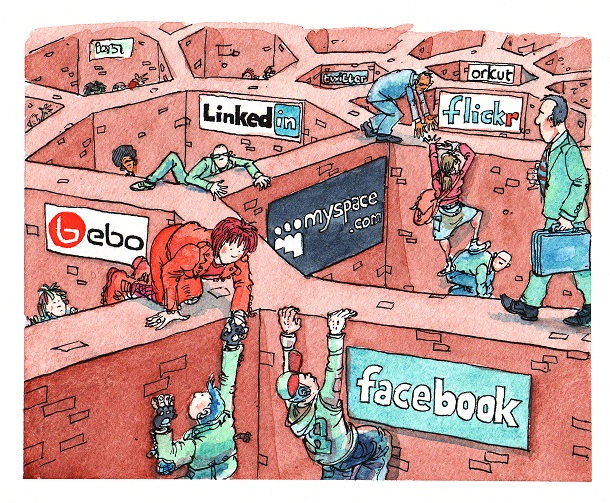
\includegraphics[width=1.0\linewidth,trim=16px 17px 12px 15px,clip]{./resources/davidsimonds.jpg}
\caption{David Simonds illustrates social networks as walled gardens due to their (by design) lock-in effects~\cite{DavidSimonds}.}
\label{fig:DavidSimonds}
\end{figure}

\subsection{Social Networks}
\section{Discussion}
\section{Future Work and Conclusion}
\section{Acknowledgments}
This work was partially supported by the European Commission under Grant No. 248296 FP7 \mbox{I-SEARCH} project.

% back to normal size Computer Modern for URLs in bibliography
\let\ttdefault\oldttdefault
\let\url\oldurl

\bibliographystyle{abbrv}
\bibliography{icmr2012}

\balancecolumns
\end{document}